%=======================================================================
%  SMN2-RescueDiff -- IEEE Transactions format, revision 2
%  All items from the reviewer report have been applied.
%  Compile with pdfLaTeX. Requires IEEEtran.cls (ships with Overleaf).
%=======================================================================
\documentclass[journal]{IEEEtran}

\usepackage{amsmath,amssymb,amsfonts}
\usepackage{mathrsfs}
\usepackage{bm}
\usepackage{graphicx}
\usepackage{url}
\usepackage{array}
\usepackage{booktabs}
\usepackage{makecell}
\usepackage[T1]{fontenc}
\usepackage[utf8]{inputenc}
\usepackage{textcomp}

\usepackage{placeins}
\usepackage[protrusion=true,expansion=false]{microtype}

% ---- typographic hygiene: no widows, no orphans, no split lines ----
\widowpenalty=10000
\clubpenalty=10000
\displaywidowpenalty=10000
\brokenpenalty=10000
\predisplaypenalty=10000
\interdisplaylinepenalty=10000
\raggedbottom

% ---- float packing: allow bottom and in-text placement and trim the
%      separation LaTeX reserves, so figures stop forcing page breaks ----
\renewcommand{\topfraction}{0.95}
\renewcommand{\bottomfraction}{0.90}
\renewcommand{\textfraction}{0.05}
\renewcommand{\floatpagefraction}{0.85}
\setlength{\textfloatsep}{8pt plus 2pt minus 2pt}
\setlength{\floatsep}{8pt plus 2pt minus 2pt}
\setlength{\intextsep}{8pt plus 2pt minus 2pt}
\setlength{\dblfloatsep}{8pt plus 2pt minus 2pt}
\setlength{\dbltextfloatsep}{8pt plus 2pt minus 2pt}
\tolerance=1800
\emergencystretch=1.6em
\hyphenation{coun-ter-screen-ing coun-ter-screen se-lec-tiv-ity
  de-sir-abil-ity con-form-er con-form-ers tran-scrip-tome
  pri-ori-ti-za-tion pri-ori-tiz-ing in-ter-pret-abil-ity
  phys-ico-chem-i-cal re-pro-duc-i-bil-ity ris-di-plam bran-a-plam
  Au-to-Dock}

% Remaining author-supplied fields are typeset in bold so they cannot be
% missed. Delete this macro once every one has been filled in.
\newcommand{\fillin}[1]{\textbf{#1}}

\begin{document}

\title{SMN2-RescueDiff: An Auditable Autoregressive Generation and RNA-Decoy Docking Pipeline for \textit{SMN2} Splicing-Modifier Prioritization}

\author{Saksham~Srivastava%
\thanks{S.~Srivastava is with Saint Francis High School, Mountain View,
CA, 94040, United States (e-mail: saksham.shubh2010@gmail.com).
ORCID ID: \mbox{0009-0007-9463-6294}.}%
\thanks{This work received no external funding. The author declares no
conflict of interest.}%
\thanks{No part of this work has been previously published or submitted
elsewhere, and no preprint has been posted.}}

\markboth{IEEE Transactions on Computational Biology and
Bioinformatics}%
{Srivastava: Auditable Generation and RNA-Decoy Screening for the
\textit{SMN2} Exon 7 Splicing Target}

\maketitle

%-----------------------------------------------------------------------
\begin{abstract}
Spinal muscular atrophy can be treated by increasing inclusion of exon
7 in \textit{SMN2} transcripts, but computational prioritization of
RNA-binding small molecules requires both target screening and difficult
off-target controls. This study introduces SMN2-RescueDiff, an auditable
pipeline that couples unconditional autoregressive SELFIES generation,
chemical filtering, five-conformer target docking, HuRDA-derived human
RNA decoy docking, and multi-factor candidate ranking. From 150{,}000
training rows, 149{,}534 valid unique ChEMBL/ZINC molecules were used;
49{,}660 unique generated strings were emitted, 40{,}477 passed chemical
filters, and 1{,}000 were exported for docking. The target campaign
completed all 2{,}500 planned jobs for 500 molecules and five fixed
\textit{SMN2} RNA conformers. The staged decoy campaign completed
14{,}259 non-dry-run AutoDock Vina jobs and yielded a uniform
$147\times97$ molecule--decoy matrix without score imputation. All 40
leading candidates had stronger mean target scores than their own
property-matched control medians; the mean enrichment was
0.729~kcal/mol and exceeded every one of 2{,}000 random cohorts. This
demonstrates reproducible target-score enrichment within the generated
population and successful operation of the staged screening
architecture. The same audit also identified an important boundary:
all conservative target--decoy gaps were negative, and redocking of four
experimental RNA--ligand complexes recovered a sub-2~\AA{} rank-1 pose
only for branaplam. Lower-RMSD modes were nevertheless sampled for
SMN-CX and risdiplam, motivating RNA-aware reranking. The contribution
is therefore a reproducible candidate-prioritization and validation
framework, not evidence that any generated molecule binds RNA, rescues
exon 7 inclusion, or has therapeutic activity.
\end{abstract}

\begin{IEEEkeywords}
Autoregressive molecular generation, molecular docking, RNA, spinal
muscular atrophy, reproducibility, virtual screening.
\end{IEEEkeywords}

%=======================================================================
\section{Introduction}
%=======================================================================
\IEEEPARstart{S}{pinal} Muscular Atrophy (SMA) patients experience
degeneration of motor neurons, resulting in debilitating muscle atrophy
and eventually full paralysis. Muscle atrophy from SMA also causes
difficulty breathing and swallowing due to degeneration of throat
muscles~\cite{aslesh2022}. SMA is a neuromuscular disorder caused by
insufficient functional survival motor neuron protein, most often due to
chromosomal deletion of the Survival Motor Neuron 1 (\textit{SMN1})
gene. Three drugs have been approved for SMA: risdiplam, an orally
administered small molecule; nusinersen (Spinraza), an antisense
oligonucleotide requiring repeated intrathecal administration; and
onasemnogene abeparvovec (Zolgensma), a single-dose gene therapy.
Current treatments do not restore mobility already lost to motor neuron
degeneration, and small-molecule splicing modifiers carry the risk of
off-target splice modulation~\cite{aslesh2022}. The
closely related \textit{SMN2} gene can partially compensate for the
disruption of \textit{SMN1}, but inefficient inclusion of exon 7 during
pre-mRNA splicing limits production of stable full-length SMN protein.
Thus, \textit{SMN2} offers a therapeutic route to increasing functional
SMN protein~\cite{aslesh2022}. The potential to restore patient mobility
makes \textit{SMN2} splicing an important therapeutic target, and the
success of small-molecule splicing modifiers has shown that RNA
processing can be pharmacologically altered to increase functional SMN
expression~\cite{chong2021}. In the SPR1NT trial, presymptomatic infants
treated with onasemnogene abeparvovec within six weeks after birth
achieved substantially better developmental outcomes than expected from
the natural history of SMA~\cite{strauss2022}. However, RNA drug targets present a
challenging drug-design problem because RNA structures are dynamic,
highly charged, and able to form binding environments that can be
difficult to distinguish computationally from unrelated RNA sites.
RNA-targeted drug discovery must account for RNA structure, ligand
recognition, and the difficulty of establishing selective interactions
with drug-like small molecules~\cite{warner2018},~\cite{childs2022},%
~\cite{haga2023}. These challenges have motivated growing interest in
RNA-targeted small-molecule discovery and machine-learning methods for
identifying RNA-binding sites and predicting RNA--ligand
interactions~\cite{haga2023}.

Generative artificial intelligence offers a way to explore chemical
space beyond pre-existing compound libraries by proposing new,
chemically plausible molecules. Recent RNA-focused computational
studies have addressed small-molecule binding-site prediction as well as
broader machine-learning strategies for RNA-targeted drug
design~\cite{xi2024},~\cite{zhou2024}. Previous work has demonstrated
the use of deep reinforcement learning and other generative approaches
for de novo molecular design and molecular-property
optimization~\cite{olivecrona2017},~\cite{liu2025}. Deep reinforcement
learning has been used to generate molecular structures and steer them
toward specified design objectives~\cite{olivecrona2017},%
~\cite{popova2018}. Reinforcement-learning-guided graph diffusion has
also been investigated for generating molecules with improved predicted
metabolic stability~\cite{liu2025}. However, the ability to generate
chemically plausible molecules does not, by itself, demonstrate
meaningful interaction with a biological target. This is an especially
important concern in RNA-focused models, where dataset biases or easily
learned physicochemical differences between positive and negative
examples can lead to shortcut learning rather than genuine recognition
of target-specific interaction patterns~\cite{wen2026}. Models developed
for protein-targeted drug discovery cannot automatically be assumed to
perform equally well for RNA targets, which require evaluation suited to
RNA--ligand interactions~\cite{karroucha2025}. Accordingly, rigorous
RNA-targeted computational discovery requires not only molecular
generation but also biologically relevant negative controls, structural
screening, selectivity evaluation, and interpretable ranking of
candidate molecules.

To address these challenges, this study developed SMN2-RescueDiff, a
computational proof-of-concept framework in which molecular generation
and biological target evaluation are treated as distinct but connected
stages. The pipeline first generates and chemically filters candidate
small molecules, then evaluates them against an independently defined
\textit{SMN2} exon 7/U1 splicing-related RNA target using multiple target
conformations, HuRDA-derived human RNA decoys, and additional off-target
counter-screens. Prioritization is performed using the Splicing Rescue
Selectivity Index (SRSI), which integrates target-docking evidence, RNA
counter-screening, splicing-related geometric proxies, chemical quality,
and off-target penalties. The main objectives were to determine whether
this staged framework could reproducibly move from molecule generation
to an auditable shortlist, whether target-score enrichment remained
after property matching and random-cohort controls, and whether
candidates with favorable average separation retained separation from
the single strongest decoy. The generator itself was deliberately
unconditional; \textit{SMN2} specificity entered only during docking and
ranking.

Docking was performed with AutoDock Vina. Its scoring function was
parameterized on protein--ligand complexes, and comparative assessments
report that pose-prediction accuracy for RNA--ligand complexes is
substantially lower than for protein targets and that current docking
methods predict RNA binders unreliably~\cite{agarwal2023},%
~\cite{gunasinghe2024}. Vina was chosen here for throughput and
reproducibility across a 15{,}000-job planned counter-screen rather than
for demonstrated RNA accuracy. Consequently, docking values below are
reported as comparative Vina scores, not binding free energies. An RNA-targeted
generative-chemistry study has combined molecular design with compound
synthesis and experimental testing, underscoring the further validation
required after computational prioritization~\cite{allen2026}.

%=======================================================================
\section{Materials and Methods}
\label{sec:methods}
%=======================================================================
SMN2-RescueDiff is a modular computational biology pipeline designed to
prioritize candidate small molecules for predicted \textit{SMN2} exon 7
splicing rescue. The pipeline is organized into six modules that
generate reproducible output files as inputs for later stages
(Fig.~\ref{fig:pipeline}): \textit{SMN2} target definition, Human RNA
Decoy Atlas construction, AI-based molecule generation, docking and
off-target counter-screening, splicing-rescue scoring and final
candidate ranking, and final virtual screening. This project is fully
computational.

\begin{figure*}[!t]
\centering
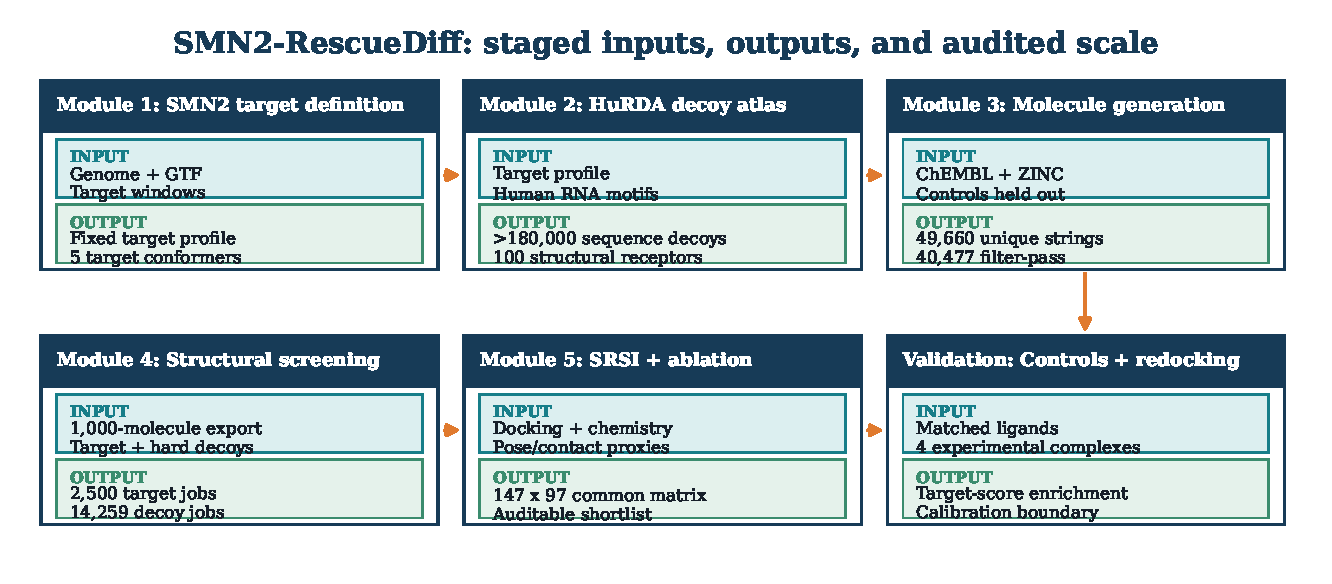
\includegraphics[width=\textwidth]{figures/Fig_pipeline.pdf}
\caption{Input-output diagram. \textit{SMN2} feature calculation and
HuRDA RNA-decoy construction establish the biological reference for
screening, while molecular generation independently produces chemically
filtered candidates. These streams converge in target docking and
off-target counter-screening. Docking, selectivity, chemical-quality,
and splicing-related proxy features are integrated through the Splicing
Rescue Selectivity Index (SRSI), followed by benchmark comparison and
candidate prioritization. Arrows indicate transfer of computational
inputs and outputs.}
\label{fig:pipeline}
\end{figure*}

%-----------------------------------------------------------------------
\subsection{Module 1: \textit{SMN2} Target Definition}

The first module defined the \textit{SMN2} exon 7 splicing-related RNA
target region, creating a reproducible reference target for all later
stages. Because \textit{SMN1} and \textit{SMN2} are highly similar
genes, the pipeline did not automatically select a target transcript
when multiple \textit{SMN2} transcript candidates were present. Instead,
an explicit \textit{SMN2} transcript ID was required in the
configuration file before execution continued. Requiring the correct
transcript reduced the risk of extracting the wrong paralog, transcript,
or exon region.

The module took two input files: a human genome FASTA file and a
matching GTF annotation file. The genome FASTA provided the genomic
sequence, while the GTF annotation file provided gene, transcript, exon,
strand, and coordinate information. The pipeline searched the annotation
file for \textit{SMN2}, enumerated transcript candidates, and required
the selected transcript ID to be written into the configuration file.

After transcript selection, the module extracted the \textit{SMN2} exon
7 region and nearby splicing-related target windows. These windows
included the exon 7 sequence, the 5$'$ splice-site region, the 3$'$
splice-site region, and additional local target windows of 21, 51, and
101 nucleotides. The 21~nt core target window was used for precise
target mapping. The 51- and 101-nt windows were used to characterize the
sequence context from which the hardest decoys were subsequently
selected. The 5$'$ and 3$'$ splice regions and the 21~nt window are the
regions the generated molecules were intended to target; the 5$'$ splice
region is the exon-intron boundary and the 3$'$ splice region is the
spliceosome acceptor. Extracted genomic sequences were converted to RNA
by substituting uracil for thymine, and the reverse complement was taken
only when the GTF strand field indicated that \textit{SMN2} lies on the
minus strand, so that the extracted sequence always corresponds to the
sense transcript.

Module 1 also calculated a target feature profile for each
\textit{SMN2} window, designed to describe the target region in a form
usable for bias-matched RNA decoy construction. The calculated features
included sequence length, nucleotide composition, A/U/G/C frequencies,
GC content, purine fraction, pyrimidine fraction, dinucleotide counts,
3-mer counts, simple splice-site-related scores, U1 complementarity
score, splice-boundary information, and positional distances relative to
exon 7. This profile constitutes the \textit{SMN2} target
``fingerprint,'' which the Human RNA Decoy Atlas then used to identify
human RNA motifs resembling the \textit{SMN2} target in sequence and
splicing-related features, so that later comparisons were made against
hard rather than trivially distinguishable negative controls. A metadata
record captured the project name, module name, selected gene, selected
transcript, input file paths, created target windows, warnings, and
limitations, so that downstream modules could trace exactly how the
\textit{SMN2} target was defined.

%-----------------------------------------------------------------------
\subsection{Module 2: HuRDA Human RNA Decoy Atlas}
\label{sec:hurda}

The second module used the Module 1 outputs as reference inputs to
construct an RNA decoy dataset. Its purpose was to test whether
generated molecules bind selectively to the \textit{SMN2} exon 7 target
or also bind similar RNA motifs elsewhere in the human transcriptome.

The atlas was specified at a transcriptome scale of over 180{,}000 RNA
motifs across eight categories: human 5$'$ splice-site decoys, human
3$'$ splice-site decoys, \textit{SMN2}-like hard decoys, exonic
regulatory windows, intronic regulatory windows, scrambled
\textit{SMN2} controls, mutated \textit{SMN2} controls, and random
bias-matched transcriptome windows. It is important to state the scope
of what was actually used: this sequence-level atlas supplied the
feature space from which decoys were selected, but only 100 decoy
sequences were converted into three-dimensional receptors and docked.
All structural selectivity results reported in this paper therefore rest
on a 100-receptor panel, not on the full sequence atlas, and the
sequence atlas contributes selection criteria rather than screening
evidence.

For every decoy motif, the same general feature types calculated in
Module 1 were recalculated, including length, nucleotide composition, GC
content, k-mer similarity, splice-site score, U1 complementarity, and
similarity to the \textit{SMN2} target profile. These sequence and
splice-related properties were used for bias matching; they were not
treated as experimentally measured RNA accessibility or secondary
structure. This allowed selection of hard, bias-matched decoys rather
than random easy controls, reducing the risk that later screening would
be evaluated only against trivially different sequences.

%-----------------------------------------------------------------------
\subsection{Module 3: AI Molecular Generation}

Module 3 generated candidate small molecules for docking and screening.
The quality-source manifest supported ChEMBL, ZINC, R-BIND 2.0 and
SMMRNA inputs, but the audited run loaded molecules only from ChEMBL and
ZINC: 74{,}558 and 74{,}976 valid unique records, respectively. The
configured R-BIND and SMMRNA paths contributed zero rows and therefore
did not provide RNA-ligand bias in this experiment. ChEMBL provides
curated drug-discovery data, while ZINC20 provides a large collection of
purchasable molecular structures for ligand
discovery~\cite{zdrazil2024},~\cite{irwin2020}. Risdiplam and branaplam
were maintained as held-out benchmark controls and were not used for
training. The combined library was validated with RDKit, canonicalized,
deduplicated, and expanded through source weights to 224{,}092 training
exposures while retaining 149{,}534 unique molecules. A baseline SMILES
n-gram generator and a character-level GRU generator were implemented,
but no baseline performance comparison is claimed here; every molecule
carried forward in this study came from the Transformer generator.

Generated SMILES strings were checked using RDKit, which determined
whether each string could be parsed into a chemically valid molecular
graph. Invalid SMILES were rejected, and valid molecules were
canonicalized and filtered on computational chemical properties. The
chemical filters included molecular weight, LogP, hydrogen bond donors,
hydrogen bond acceptors, rotatable bonds, formal charge, ring count,
aromatic ring count, QED drug-likeness, Lipinski rule compliance, PAINS
alerts, novelty, and diversity. PAINS substructure alerts were used as
screening flags for possible assay-interference liability rather than as
experimental evidence that a candidate interferes with an
assay~\cite{baell2010}. Quantitative estimate of drug-likeness (QED) was
included as a calculated descriptor of molecular properties associated
with drug-like compounds~\cite{bickerton2012}.

\subsubsection{Autoregressive molecular generation}
The production generator was an autoregressive Transformer operating on
SELFIES tokens. After cleaning, canonicalization, and duplicate removal,
the SMILES were converted to SELFIES, an alternative string
representation of molecular structure. Each SELFIES string was split
into molecular symbols, mapped to token identifiers, and supplied with
start and end tokens. The Transformer learned to predict the next
SELFIES token from the preceding tokens using causal self-attention.
SELFIES was selected because its grammar is designed to produce valid
molecular structures from valid SELFIES strings~\cite{krenn2020}.

The architecture comprised six layers, eight attention heads,
384-dimensional embeddings, sinusoidal positional encodings, a
1{,}536-dimensional feed-forward network, and a dropout rate of 0.1.
Training used AdamW with a learning rate of 0.0005, a weight decay of
$10^{-5}$, gradient clipping at a norm of 1.0, a batch size of 128, and
next-token cross-entropy loss excluding padding positions, for up to 10
epochs with early stopping at a patience of six epochs. A random seed of
42 was used, and 10\% of the tokenized sequences were reserved for
validation.

Generation began with a start token and proceeded one SELFIES token at a
time until an end token was sampled or 160 sampling steps had been
completed. Sampling used a temperature of 0.78, top-$k$ filtering with
$k = 50$, and top-$p$ filtering with $p = 0.95$. The sampled token
identifiers were reconstructed into SELFIES strings and converted to
SMILES using the SELFIES decoder. These decoded SMILES were parsed,
sanitized, and canonicalized with RDKit before duplicate removal,
chemical-property filtering, and candidate prioritization. SELFIES
therefore served as the model's training and generation representation,
while SMILES served as the format for subsequent molecular processing
and export. \textit{SMN2} specificity was assessed downstream through
target-conformer docking, HuRDA RNA counter-screening, and SRSI ranking;
the generator received molecular tokens without \textit{SMN2} sequence
conditioning.

The autoregressive objective is given in~\eqref{eq:autoregressive}:
\begin{equation}
\begin{aligned}
p_{\theta}(x_{1:T}) &= \prod_{t=1}^{T} p_{\theta}(x_{t} \mid x_{<t}),\\[4pt]
\mathscr{L}_{\mathrm{CE}} &= -\,\frac{\displaystyle\sum_{n,t} m_{nt}
\log p_{\theta}(x_{nt} \mid x_{n,<t})}{\displaystyle\sum_{n,t} m_{nt}},
\end{aligned}
\label{eq:autoregressive}
\end{equation}
where $x_{nt}$ is token $t$ of training molecule $n$ and $m_{nt}$
excludes padding tokens.

%-----------------------------------------------------------------------
\subsection{Module 4: Docking and Off-Target Counter-Screening}

This module computed comparative docking scores and selectivity proxies
for candidate molecules at the \textit{SMN2} exon 7 splicing-related RNA
target and selected human RNA decoys from HuRDA.

Molecular docking requires a three-dimensional receptor structure. A
hard-decoy panel selected from HuRDA was converted into predicted 3D RNA
receptor structures using RNA Composer, then prepared as PDBQT
receptors for structural counter-screening. Candidate--receptor poses
and docking scores were generated using AutoDock Vina, whose original
search and scoring approach and subsequent software extensions have been
described in the literature~\cite{trott2010},~\cite{eberhardt2021}. All
decoy docking scores were non-dry-run Vina outputs, and pose files were
generated for molecule-decoy pairs.

The docking module calculated \textit{SMN2} target docking scores, decoy
docking scores, and target-to-decoy selectivity metrics. Because more
negative Vina values are treated as more favorable by the scoring
function, selectivity was computed so that a larger positive gap
corresponds to a more favorable target score relative to decoys.
Candidates showing favorable \textit{SMN2} scores and less favorable
decoy scores advanced to the splicing-rescue scoring module.

%-----------------------------------------------------------------------
\subsection{Module 5: Splicing Rescue Selectivity Index and Ranking}

Module 5 combined docking and chemical-property results into the SRSI.
For each molecule, the HuRDA decoy score was computed as a biologically
weighted mean across the receptors that were successfully scored.
Subtracting the mean \textit{SMN2} conformer Vina score from this
quantity yielded the weighted selectivity gap; because more negative
Vina scores are more favorable within the scoring function, a larger
positive gap corresponded to a more favorable comparative score for
\textit{SMN2}. A conservative gap was also calculated by comparing the
strongest-scoring decoy with the molecule's least favorable
\textit{SMN2} conformer, and decoy coverage recorded the fraction of
planned comparisons that produced usable scores~\eqref{eq:selectivity}.
Failed docking jobs were not assigned estimated scores.

For successfully scored decoys $\mathscr{D}_{i}$, with biological
weights $w_{j}$:
\begin{equation}
\begin{aligned}
\overline{E}_{i}^{D,w} &=
\frac{\displaystyle\sum_{j \in \mathscr{D}_{i}} w_{j} E_{ij}^{D}}
     {\displaystyle\sum_{j \in \mathscr{D}_{i}} w_{j}},\\[4pt]
\Delta_{i}^{w} &= \overline{E}_{i}^{D,w} - \overline{E}_{i}^{T},\\[4pt]
\Delta_{i}^{\mathrm{conservative}} &=
\min_{j \in \mathscr{D}_{i}} E_{ij}^{D} - E_{i,\mathrm{worst}}^{T},\\[4pt]
\mathrm{Coverage}_{i} &= \frac{|\mathscr{D}_{i}|}{M},
\end{aligned}
\label{eq:selectivity}
\end{equation}
where $M$ is the planned number of decoys. Weights $w_{j}$ were read
from the decoy annotation; decoys without a recorded weight defaulted to
$w_{j} = 1$, which is a scoring convention rather than a statement of
biological importance.

\subsubsection{Splicing-rescue proxy}
The splicing-rescue proxy combined weighted target-docking,
splice-region and U1-related, and contact-support components, together
with pose-based support when usable pose evidence was available or
feature-based support when it was not. Penalties for missing pose
evidence, splice-site occlusion, and off-target risk were then applied;
the result was scaled by the configured denominator and constrained to
the interval $[0,1]$:
\begin{equation}
R_{i} = \mathrm{clip}_{[0,1]}\!\left[\frac{1}{D}
\begin{aligned}[t]
 \Bigl(&\textstyle\sum_{k \in \mathscr{P}} a_{k} u_{ik}
 + 2 m_{i} F_{i}\\
 &+ 1.5\,(1 - m_{i}) V_{i}\\
 &- b_{C} C_{i} - b_{O} O_{i} - b_{m} m_{i} \Bigr)
\end{aligned}
\right],
\label{eq:rescue}
\end{equation}
in which $u_{ik}$ are positive support components (target-docking,
landmark/U1 support and contact proxies); $F_{i}$ is feature-based
support; $V_{i}$ is the pose-support score; $m_{i}$ indicates missing or
unusable pose evidence; $C_{i}$ is the splice-site occlusion penalty;
$O_{i}$ is off-target risk; and $a_{k}, b_{C}, b_{O}, b_{m}$ are
configured weights. The implementation uses
\begin{equation*}
D = \max\!\left(10^{-9},
\sum_{w \in \text{configured rescue weights}} |w| + 2 \right).
\end{equation*}

The configured positive weights were 2.0 for beneficial-landmark
proximity, 2.0 for U1 support, 1.5 for exon-7-boundary support, 1.5 for
target score, 1.0 for contact density, 0.8 for the hydrogen-bond proxy,
and 0.7 for the stacking proxy. Penalty weights were 2.0 for occlusion,
1.5 for off-target risk, and 0.5 for missing pose evidence. A usable
pose contributed $1.5V_i$; a missing pose contributed $2F_i$.

Contact features were atom-pair proxies with fixed cutoffs: 4.5~\AA{}
for a close contact, 3.5~\AA{} for a hydrogen-bond-like pair, and
5.0~\AA{} for a carbon--carbon stacking-like pair. For $N_i$ ligand
atoms, contact density was
$\min(1,n_{\mathrm{close}}/(4N_i))$; hydrogen-bond and stacking scores
were $\min(1,n/(0.5N_i))$; and
$V_i=\mathrm{clip}_{[0,1]}(0.45d_i+0.30h_i+0.25s_i)$. The implementation
did not map every receptor atom to a nucleotide landmark. If a U1 or
5$'$-site label was present, beneficial contacts were assigned as
$\lfloor0.75n_{\mathrm{close}}\rfloor$; if donor or acceptor labels were
present, caution contacts were assigned as
$\lfloor0.35n_{\mathrm{close}}\rfloor$, and
$C_i=n_{\mathrm{caution}}/\max(1,n_{\mathrm{close}})$. These are explicit
engineering proxies, not experimentally observed contacts or mechanistic
splicing measurements.

\subsubsection{SRSI standardization and integration}
For the final SRSI, continuous features were standardized across the
scored candidate cohort and combined using the configured weights. The
Lipinski-pass and PAINS-alert indicators were included without
standardization. For a scoring feature $x$:
\begin{equation*}
\begin{aligned}
z_{i}(x) &= \frac{x_{i} - \mu_{x}}{\sigma_{x}}, \qquad
\mu_{x} = \frac{1}{n}\sum_{i} x_{i},\\[4pt]
\sigma_{x} &= \sqrt{\frac{1}{n}\sum_{i}(x_{i} - \mu_{x})^{2}}.
\end{aligned}
\end{equation*}

The complete scoring equation is
\begin{equation}
\begin{aligned}
S_{i} ={}& w_{B} z_{i}\!\left(-E^{T}\right) + w_{R} z_{i}(R)
         + w_{\Delta} z_{i}(\Delta^{w}) + w_{Q} z_{i}(Q)\\
      &+ w_{L} I_{i}^{L} + w_{P} z_{i}(P) - w_{O} z_{i}(O)
         - w_{A} z_{i}(A)\\
      &- w_{H} I_{i}^{H} - w_{C} z_{i}(C),
\end{aligned}
\label{eq:srsi}
\end{equation}
with $-E^{T}$ target-docking strength ($w_{B} = 1.0$); $R$ rescue proxy
($w_{R} = 2.0$); $\Delta^{w}$ weighted selectivity gap
($w_{\Delta} = 1.5$); $Q$ QED ($w_{Q} = 0.7$); $I^{L}$ Lipinski-pass
indicator ($w_{L} = 0.4$); $P$ pre-docking score ($w_{P} = 0.5$); $O$
off-target risk ($w_{O} = 1.5$, subtracted); $A$ lower-is-better SA
score ($w_{A} = 0.5$, subtracted); $I^{H}$ PAINS-alert indicator
($w_{H} = 1.0$, subtracted); and $C$ occlusion penalty ($w_{C} = 1.2$,
subtracted).

%-----------------------------------------------------------------------
\subsection{Module 6: Final Virtual Screening Protocol}

Module 6 specified the staged evaluation applied to the generated
candidates. Rather than relying on a single docking score, candidates
passed through target-conformer screening, RNA counter-screening,
ensemble-aware selectivity analysis, additional off-target screening,
and benchmarking against established \textit{SMN2} splicing modifiers,
and were required to satisfy several independent computational criteria
before advancement.

\subsubsection{Target-conformer robustness screening}
Five fixed \textit{SMN2} target conformers were prepared and used as a
receptor ensemble. A pilot $10 \times 5$ experiment preceded full
screening of 500 candidate molecules against all five conformers. For
each molecule the pipeline calculated mean, median, best, and worst
target Vina scores, standard deviation across conformers, and total
target-score range, and prioritized candidates by more favorable
worst-conformer score, more favorable mean score, and lower variation
across the conformational ensemble. Molecules requiring lower-confidence
rigid-tree repair during the target screen were excluded from standard
advancement, preventing repaired docking artifacts from influencing
selection. For $K = 5$ conformers:
\begin{equation}
\begin{aligned}
\overline{E}_{i}^{T} &= \frac{1}{K}\sum_{c=1}^{K} E_{ic}^{T},
\qquad
E_{i,\mathrm{worst}}^{T} = \max_{c} E_{ic}^{T},\\[4pt]
s_{i}^{T} &= \sqrt{\frac{1}{K - 1}
\sum_{c=1}^{K}\left(E_{ic}^{T} - \overline{E}_{i}^{T}\right)^{2}}.
\end{aligned}
\label{eq:conformer}
\end{equation}

\subsubsection{HuRDA RNA counter-screening}
The 150 conformer-robust molecules were evaluated against 100 human RNA
decoy receptors derived from the HuRDA atlas. To reduce computational
load while preserving the complete receptor panel, the experiment was
divided into two docking runs: 150 molecules against 53 receptors and
150 molecules against the remaining 47 receptors. This stage was
designed to move beyond an absolute target score and evaluate
comparative RNA docking behavior: a molecule receiving a favorable
\textit{SMN2} score but equally favorable scores on many unrelated human
RNA structures is less compelling than one with a wider target--decoy
score gap. Only successfully completed docking
calculations were retained in the merged dataset; failed jobs were not
assigned artificial or imputed scores.

\subsubsection{Ensemble-aware selectivity analysis}
\label{sec:ensemble}
Candidates were ranked lexicographically on five criteria in order:
larger weighted mean selectivity gap, larger conservative selectivity
gap, reduced predicted off-target risk, a more favorable mean
\textit{SMN2} score, and lower variation across the five \textit{SMN2}
conformers. A
later criterion is consulted only when every earlier criterion ties. The
conservative selectivity calculation imposed a stricter test than
comparison of average scores alone: it evaluated whether \textit{SMN2}
remained the preferred predicted target when the candidate's least
favorable \textit{SMN2} conformer was compared with its strongest
apparent interaction among off-target RNAs. This reduced the
150-molecule cohort to the top 40 candidates.

\subsubsection{Cross-target off-target screening}
Each of the top 40 candidates was evaluated against 20 additional
target-decoy receptors, producing 800 planned docking calculations, to
identify candidates that maintained favorable \textit{SMN2}-directed
performance while minimizing strong predicted interactions with
additional non-primary targets. This stage distinguished molecules that
appeared promising primarily because of a favorable target score from
molecules that retained a more favorable computational specificity
profile across multiple target classes.

\subsubsection{Benchmark comparison with known \textit{SMN2} splicing
modifiers}
Risdiplam and branaplam were processed under the same protocol as the
generated candidates, because a credible computational prioritization
pipeline should be able to recognize established \textit{SMN2} splicing
modifiers before predictions for newly generated molecules are
interpreted. Benchmark compounds were compared on target engagement,
selectivity, and developability. Developability was scored with
desirability functions rather than raw min--max normalization, so that
each value is interpretable against a fixed, prespecified acceptance
window instead of against the other two compounds. For a preferred
interval $[a,b]$ with author-set tolerances $\alpha$ and $\beta$,
\begin{equation}
d(x) =
\begin{cases}
0, & x \le a-\alpha,\\[2pt]
\dfrac{x-(a-\alpha)}{\alpha}, & a-\alpha < x < a,\\[6pt]
1, & a \le x \le b,\\[2pt]
\dfrac{(b+\beta)-x}{\beta}, & b < x < b+\beta,\\[6pt]
0, & x \ge b+\beta,
\end{cases}
\label{eq:desirrange}
\end{equation}
and for one-sided criteria with target $T$ and zero-credit bound $L$ or
$U$,
\begin{equation}
d_{\uparrow}(x) = \mathrm{clip}\!\left(\frac{x-L}{T-L},0,1\right),
\quad
d_{\downarrow}(x) = \mathrm{clip}\!\left(\frac{U-x}{U-T},0,1\right).
\label{eq:desironesided}
\end{equation}
Per-metric desirabilities were aggregated as a weighted geometric mean,
\begin{equation}
D = \left(\prod_{m=1}^{M} d_{m}^{\,\omega_{m}}\right)^{1/\sum_{m}\omega_{m}},
\label{eq:geomean}
\end{equation}
so that a metric scoring $d_{m} = 0$ drives $D$ to zero. All anchors,
tolerances, and weights are given in Table~\ref{tab:desir}; no parameter
was fitted to the compared compounds.

The benchmark strategy evaluated more than docking score alone.
Native-pose redocking was carried out against four experimentally
determined RNA--ligand complexes, including risdiplam and branaplam,
using five seeds, 20 retained modes per run, and symmetry-corrected
heavy-atom RMSD. Pose recovery and native-contact overlap were analyzed
separately from candidate ranking, as reported in
Section~\ref{sec:res-redock}. Benchmark controls were not used for model
training.

\subsection{Stage C.5: Matched Ligand Decoy Controls}
\label{sec:ligandcontrols}
The HuRDA panel of Section~\ref{sec:hurda} varies the receptor while
holding the ligand fixed, and therefore cannot distinguish a candidate
that engages \textit{SMN2} specifically from one that docks well
because of its size and physicochemical profile. Stage C.5 applies the
complementary control: the receptor ensemble is held fixed and the
ligand is varied, by comparing each ranked candidate with
property-matched decoy ligands drawn from the same generated
population.

Controls were selected from the 500-molecule target-ensemble population
after removing the 40 ranked candidates and any exact structural
duplicates, leaving a pool of 460. Nine descriptors were standardized
across the combined candidate and control population---molecular
weight, cLogP, hydrogen-bond donors and acceptors, tPSA, rotatable
bonds, formal charge, QED and a synthetic-accessibility proxy---and
each candidate was matched to its ten nearest controls by Euclidean
distance in that standardized space. A Morgan fingerprint guard
(radius 2, 2048 bits) excluded any control with Tanimoto similarity
above 0.6 to its candidate, so that matched pairs share physicochemical
profile without sharing scaffold. Controls could be reused across
candidates, and reuse counts are reported. For candidate $i$ with
matched-control set $\mathscr{C}_{i}$, the target enrichment gap is
\begin{equation}
g_{i} = \operatorname*{median}_{c \in \mathscr{C}_{i}}
        \overline{E}_{c}^{T} \;-\; \overline{E}_{i}^{T},
\label{eq:ligandgap}
\end{equation}
so that $g_{i} > 0$ means the candidate receives a more favorable mean
\textit{SMN2} score than the median of its own matched controls. The
40 candidate matched sets were treated as the independent units.
Confidence intervals were obtained by bootstrap over those sets
(10{,}000 resamples), and significance by a random sign-flip
permutation test on the candidate-level gaps (20{,}000 permutations),
both under seed 61453. Stage C.5 performed no new docking: it reuses
the five-conformer target results of~\eqref{eq:conformer}, and no
missing score was repaired or imputed.

%=======================================================================
\section{Results}
%=======================================================================

\subsection{Generation and chemical triage}
\label{sec:res-generation}

The audited generation run converted a broad chemical-language model
into a manageable docking cohort (Table~\ref{tab:generation}). Of
150{,}000 source rows, 149{,}534 parsed as valid, unique molecules and
466 were rejected. Source weighting produced 224{,}092 training
exposures without altering the unique-molecule record. Training ran for
10 epochs; final training and validation cross-entropy losses were
0.6287 and 0.5722, respectively.

The run requested 50{,}000 samples and emitted 49{,}660 unique generated
strings. Every emitted string parsed with RDKit, while canonicalization
left 49{,}489 unique molecular graphs. Chemical-quality filters retained
40{,}477 molecules and rejected 9{,}183. Of the retained set, 40{,}406
were novel under the run's approximate comparison with the first
20{,}000 canonical training molecules; this is not a full-corpus novelty
estimate. Diversity-aware
selection exported 1{,}000 candidates for docking, representing 977
recorded scaffold labels. Across 50{,}000 sampled fingerprint pairs,
the mean and median Morgan Tanimoto similarities were 0.121 and 0.115,
respectively, indicating that the exported cohort was not dominated by
near-duplicate structures. A post hoc audit against the two held-out
splicing controls found no filtered or exported candidate above the
prespecified Tanimoto exclusion threshold of 0.70. The original run
tracked branaplam alone; adding risdiplam to the audit did not rewrite
the historical generation output.

\begin{table}[!t]
\caption{Audited Molecule-Generation and Selection Counts}
\label{tab:generation}
\centering
\footnotesize
\setlength{\tabcolsep}{4.5pt}
\renewcommand{\arraystretch}{1.15}
\begin{tabular}{@{}lr@{}}
\toprule
\textbf{Stage} & \textbf{Observed count}\\
\midrule
Source rows inspected & 150{,}000\\
Valid unique training molecules & 149{,}534\\
Invalid source rows & 466\\
Weighted training exposures & 224{,}092\\
Unique generated strings emitted & 49{,}660\\
Unique valid canonical molecules & 49{,}489\\
Molecules passing chemical filters & 40{,}477\\
Molecules rejected by filters & 9{,}183\\
Candidates exported for docking & 1{,}000\\
Recorded scaffolds in docking export & 977\\
\bottomrule
\end{tabular}
\end{table}

\begin{figure}[!t]
\centering
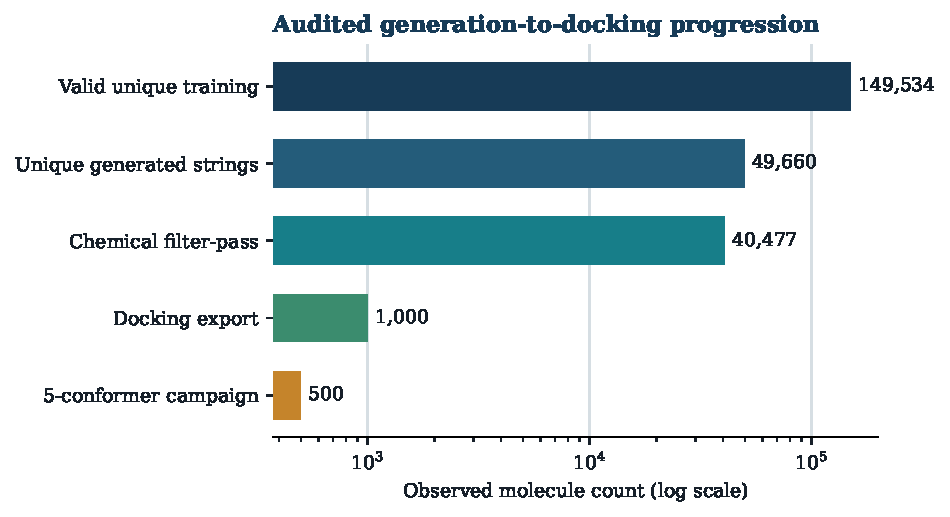
\includegraphics[width=\columnwidth]{figures/Fig_generation_audit.pdf}
\caption{Audited progression from source-library validation through
generation, chemical filtering, and diversity-aware docking export.
Counts are observed pipeline outputs, not expected or back-filled
targets. The 500-molecule structural campaign was selected from the
1{,}000-molecule docking export.}
\label{fig:generation}
\end{figure}

\subsection{Docking campaign and data completeness}

The five-conformer \textit{SMN2} target screen completed all 2{,}500
planned ligand--conformer jobs across the 500 generated candidates,
producing a complete target matrix with no missing entries. The
completed dataset was verified to contain 500 unique molecules, five
unique conformers, no duplicate molecule-conformer pairs, and five
completed conformer scores for every molecule. Two molecules required
rigid-tree repair during ligand preparation; these are retained with a
reduced-confidence flag, and their scores are reported but are not
treated as having the same confidence as those of the remaining 498.
This screen reduced the 500-molecule set to 150 conformer-robust
candidates, which were frozen with cryptographic checksums to preserve
the exact target-screening outputs used downstream.

The HuRDA counter-screen was designed as 150 molecules against 100
decoys and executed as two panels of 53 and 47 receptors, for 15{,}000
intended molecule--decoy pairs. Of these, 14{,}259 completed
successfully. The 741 jobs that did not launch are fully attributable to
unavailable docking inputs rather than to any docking outcome: three
decoy receptors could not be prepared in PDBQT format, and three ligands
could not be converted from their stored structures. Applying
inclusion--exclusion yields $(3)(150) + (3)(100) - (3)(3) = 741$, where
the final term removes the nine pairs missing both a ligand and a
receptor. The preflight check reports 750 input problems for these 741
jobs, because those nine pairs are counted twice; the two figures are
therefore consistent, not contradictory.

Because these failures arise from structural-input issues, no score was
imputed for the affected pairs and no placeholder score was
substituted. Global coverage is therefore $14{,}259/15{,}000 = 95.06\%$,
with no duplicate molecule--decoy pairs in the merged table. The
surviving data are not ragged: 147 of the 150 molecules retain an
identical, complete 97-decoy panel, so every ranking comparison is made
on a common decoy set. The remaining three molecules have zero decoy
coverage, are labeled insufficient decoy evidence, and are excluded from
ranking while their identities are preserved in the output. Each
evaluable molecule is thus assessed on 97\% of its intended panel. The
cross-target screen completed all 800 planned $40 \times 20$ docking
calculations and passed computational validation checks.

\subsection{Selectivity profile of the leading candidates}
\label{sec:res-selectivity}

The 147 evaluable candidates were ranked by the lexicographic rule of
Section~\ref{sec:ensemble}; this ensemble-aware selectivity stage is
referred to as Stage C, and the matched-control audit built on its
output as Stage C.5. Fig.~\ref{fig:stagec} presents the ten
highest-ranked candidates. Their weighted selectivity gaps ranged from
6.177 to 6.622~kcal/mol, indicating favorable average separation within
the evaluated cohort. However, all conservative gaps were negative
($-2.607$ to $-0.367$~kcal/mol): for every candidate, at least one decoy
scored more favorably than that candidate's least favorable
\textit{SMN2} conformer. None of the ten candidates met the prespecified
thresholds for mean target Vina score, weighted selectivity gap,
conservative gap, or off-target risk. The pattern is not confined to
the tabulated ten. Across all 147 evaluable molecules the conservative
gap is negative without exception, ranging from $-3.235$ to
$-0.367$~kcal/mol with a median of $-1.950$ and an interquartile range
of $[-2.304, -1.718]$, while the weighted gap over the same 147 spans
only 5.274 to 6.622~kcal/mol. Favorable mean separation
therefore coexists with a lack of worst-case separation in every
case, and a pipeline reporting only the mean gap would have assigned all
ten an unsupported selectivity interpretation.

The off-target risk index takes the identical value 0.657216 for five of
the ten candidates and 0.657216 or 0.653608 for six. Such exact ties
indicate that the index saturates at a ceiling imposed by its clipped
component terms rather than resolving differences among these
candidates. Because the ranking is lexicographic, this near-degeneracy
in the third criterion has almost no influence on the final order, which
is determined in practice by the continuous weighted gap alone.
MolGen\_048239 illustrates the consequence: it ranks sixth on the
primary criterion, yet carries both the least negative conservative gap
($-0.367$~kcal/mol) and the lowest off-target risk index (0.461) of the
ten. Under the stated ordering this profile confers no ranking
advantage.

\begin{figure}[!t]
\centering
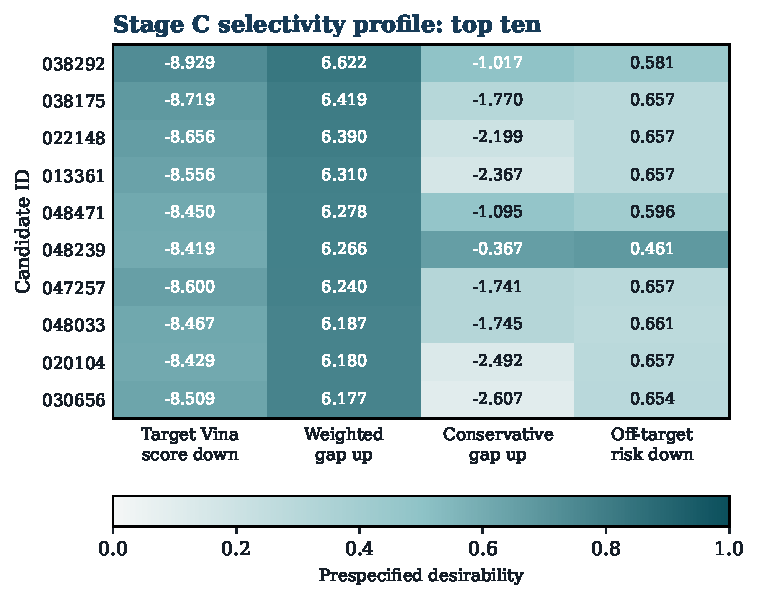
\includegraphics[width=\columnwidth]{figures/Fig_stageC_top10_heatmap.pdf}
\caption{Selectivity profile of the ten top-ranked candidates, ordered
by the lexicographic rule of Section~\ref{sec:ensemble}. Each cell
reports the measured value and is shaded by its desirability
$d \in [0,1]$ with respect to the acceptance target for that metric,
computed from~\eqref{eq:desironesided} with the anchors and acceptance
targets given in Table~\ref{tab:desir}. Arrows give the optimization direction:
$\downarrow$ smaller-is-better, $\uparrow$ larger-is-better.}
\label{fig:stagec}
\end{figure}

\subsection{Benchmark comparison}
\label{sec:res-bench}

The top-ranked generated candidate, MolGen\_038292, was compared with
risdiplam and branaplam on target scoring, RNA selectivity, and
developability (Fig.~\ref{fig:bench}). It showed the most favorable mean
target Vina score ($-8.929$ versus $-8.613$ and $-8.321$~kcal/mol),
the largest weighted selectivity gap (6.622 versus 6.309 and
6.071~kcal/mol), the lowest off-target risk index (0.581 versus 0.664
and 0.600), and the smallest fraction of decoys scoring more strongly
than the target (0.093 versus 0.124 and 0.165).

MolGen\_038292 was therefore competitive with the benchmark controls on
several outputs of the same computational protocol, which supports its
retention as a follow-up candidate. These are not clinical-superiority
claims. First, all three compounds fall outside every author-defined
acceptance window in the target and selectivity blocks. Because this
includes two established splicing modifiers, the windows function as
strict exploratory triage criteria rather than calibrated biological
decision thresholds. Second, MolGen\_038292 has a molecular weight of 504.0~Da against
401.5 and 393.5~Da for risdiplam and branaplam. AutoDock Vina scores
scale with ligand heavy-atom count, so a $0.32$--$0.61$~kcal/mol
advantage over compounds roughly 100~Da smaller is of the magnitude
expected from size alone, and ligand-efficiency normalization is
required before any target-score advantage can be interpreted. Third, several of
the candidate's physicochemical properties fall outside the preferred
ranges, and its overall desirability is 0.626, lower than risdiplam
(0.656) and branaplam (0.663). The benchmark therefore identifies a
computationally competitive generated molecule while also showing why
the pipeline must retain developability, size, and calibration checks.

\begin{figure}[!t]
\centering
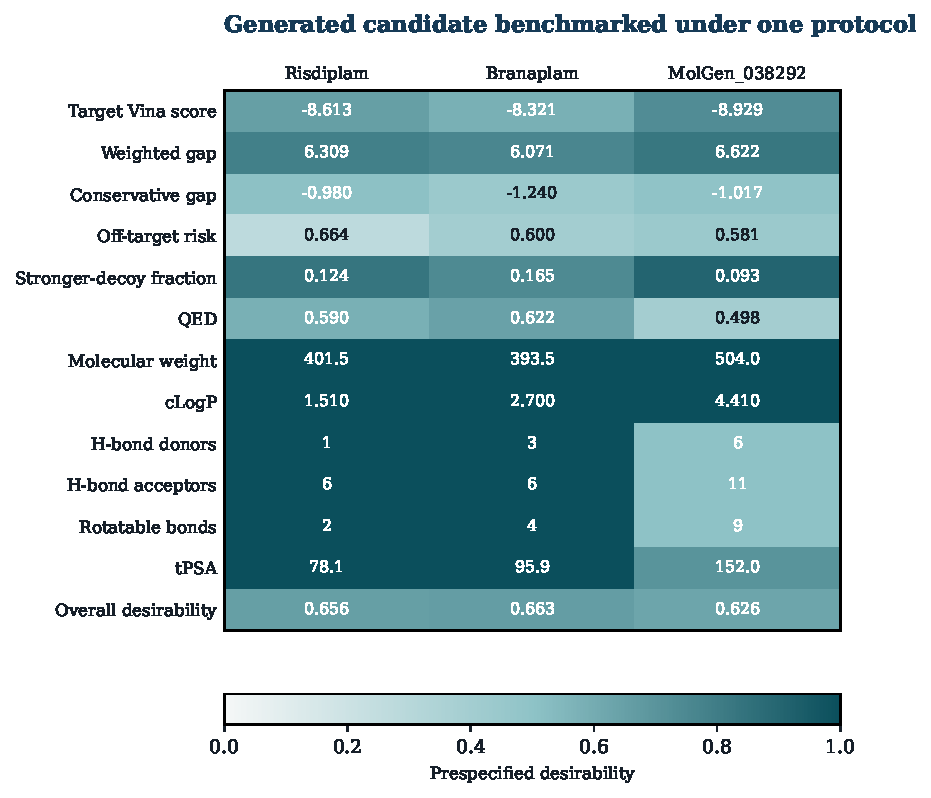
\includegraphics[width=\columnwidth]{figures/Fig_benchmark_heatmap.pdf}
\caption{Multi-objective benchmark of the top-ranked generated candidate
against two clinical-stage \textit{SMN2} splicing modulators, grouped
into target scoring, selectivity and developability. Each cell
reports the measured value and is shaded by its desirability
$d \in [0,1]$ from~\eqref{eq:desirrange} and~\eqref{eq:desironesided},
with anchors and the acceptance window for each metric given in
Table~\ref{tab:desir}. The bottom row is the overall desirability $D$
of~\eqref{eq:geomean}. Reference-compound descriptors are literature
values (PubChem CID 118513932; branaplam free base,
C$_{22}$H$_{27}$N$_{5}$O$_{2}$).}
\label{fig:bench}
\end{figure}

\begin{table}[!htbp]
\caption{Desirability Anchors, Tolerances and Weights Used in
Fig.~\ref{fig:stagec} and Fig.~\ref{fig:bench}}
\label{tab:desir}
\centering
\footnotesize
\setlength{\tabcolsep}{3.5pt}
\renewcommand{\arraystretch}{1.2}
\begin{tabular}{@{}llll@{}}
\toprule
\textbf{Metric} & \textbf{Form} & \textbf{Parameters} &
$\bm{\omega}$\\
\midrule
Mean target Vina score      & $d_{\downarrow}$ & $T=-10$, $U=-6$ & 3.0\\
Weighted selectivity gap    & $d_{\uparrow}$   & $L=0$, $T=8$    & 3.0\\
Conservative gap            & $d_{\uparrow}$   & $L=-3$, $T=1$   & 2.5\\
Off-target risk index       & $d_{\downarrow}$ & $T=0.30$, $U=0.80$ & 2.5\\
Stronger-decoy fraction     & $d_{\downarrow}$ & $T=0.05$, $U=0.50$ & 1.5\\
QED                         & $d_{\uparrow}$   & $L=0.30$, $T=0.80$ & 2.0\\
Molecular weight (Da)       & $d$ & $[220,520]$, $\alpha=70$, $\beta=80$ & 1.0\\
cLogP                       & $d$ & $[0,4.5]$, $\alpha=\beta=1.0$ & 1.0\\
H-bond donors               & $d$ & $[0,5]$, $\alpha=0$, $\beta=2$ & 0.75\\
H-bond acceptors            & $d$ & $[2,10]$, $\alpha=\beta=2$ & 0.75\\
Rotatable bonds             & $d$ & $[0,8]$, $\alpha=0$, $\beta=2$ & 0.75\\
tPSA (\AA$^2$)              & $d$ & $[35,140]$, $\alpha=15$, $\beta=40$ & 1.0\\
\bottomrule
\end{tabular}
\end{table}

\subsection{Matched ligand decoy control enrichment}
\label{sec:res-ligand}

Stage C.5 compared the 40 highest-ranked candidates with
property-matched decoy ligands under the protocol of
Section~\ref{sec:ligandcontrols}. Matching assigned 400
candidate--control pairs drawn from 183 distinct control molecules, ten
to each candidate. The match is close on physicochemical profile and
distant on structure: the mean absolute standardized difference does
not exceed 0.67 on any of the nine descriptors, while the largest
candidate--control Tanimoto similarity observed is 0.338, with a mean
of 0.124. No control exceeded the 0.6 similarity guard, so no
relaxation of the threshold was required.

Every one of the 40 candidates received a more favorable mean
\textit{SMN2} conformer score than the median of its own matched controls
(Fig.~\ref{fig:ligand}). The mean target enrichment gap
of~\eqref{eq:ligandgap} is 0.729~kcal/mol, with a bootstrap 95\%
confidence interval of $[0.660, 0.802]$; the median is 0.686, with a
bootstrap 95\% confidence interval of $[0.620, 0.835]$. A random sign-flip permutation test on
the candidate-level gaps returns $p \le 5.0 \times 10^{-5}$, the
resolution limit of 20{,}000 permutations, since no permutation reached
the observed statistic; the paired effect size is $d_{z} = 3.15$.

This is the one comparison in the study in which the generated
candidates separate from a control set, and it isolates a specific
claim: the target scores are not explained by molecular size or
drug-likeness, because the controls match on both. It does not
establish \textit{SMN2} selectivity, which is what the decoy receptor
panel tests and what Section~\ref{sec:res-selectivity} reports as
failing. Nor is the control set independent of the generator: the
controls come from the same 500-molecule population and inherit its
chemistry, so the comparison measures enrichment within that population
rather than against an external library.

A further confound is that the controls are not independent of the
selector either. The first lexicographic criterion is the weighted
selectivity gap of~\eqref{eq:selectivity}, which a molecule raises by
receiving a more favorable target score, so the 40 candidates were chosen
partly for the quantity Stage C.5 then measures. Descriptor matching
removes size and drug-likeness as explanations but cannot remove this
one. To quantify it, the protocol of Section~\ref{sec:ligandcontrols}
was rerun on 2{,}000 cohorts of 40 molecules drawn at random from the
460 unselected molecules, each matched to ten controls from the
remainder under identical rules, including the Tanimoto guard. Every
cohort found a full complement of controls. The random cohorts are
centered on zero enrichment (mean $-0.049$~kcal/mol, standard deviation
0.099, median $-0.056$), with a 99th percentile of 0.224 and a largest
cohort mean of 0.367. The observed 0.729 lies 7.84 standard deviations
above the null mean and above all 2{,}000 random cohorts
($p \le 5.0 \times 10^{-4}$, the resolution limit of the draw), so the
enrichment is not a sampling artifact.

That null varies the cohort at random, however, and therefore does not
isolate selection by target score, which is what the first
lexicographic criterion rewards. A second control addresses it directly:
a cohort of the 40 molecules with the most favorable mean target score
alone, with no decoy or selectivity term, matched under the same
protocol. That cohort enriches at least as much as the ranked one
(median 0.723 against 0.686~kcal/mol, mean 1.016 against 0.729, 40 of 40
positive in both), and shares 35 of its 40 members. The enrichment is
therefore a consequence of selecting for favorable target scores. The matched
controls establish that this is not an artifact of molecular size or
drug-likeness, and the random null that it is not chance, but neither
shows that the multi-objective rule contributes anything beyond what
ranking on target score alone would deliver.

\begin{figure}[!t]
\centering
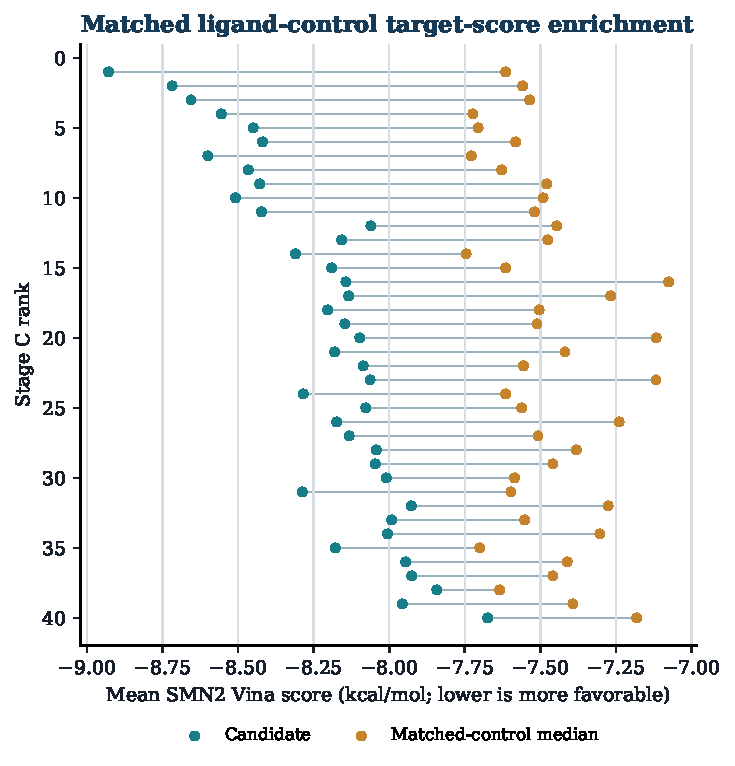
\includegraphics[width=\columnwidth]{figures/Fig_ligand_control_enrichment.pdf}
\caption{Matched ligand decoy control enrichment for the 40
highest-ranked candidates, ordered by Stage C selectivity rank. Each
row pairs one candidate with the median of its ten property-matched
controls; the horizontal segment is the target enrichment gap
of~\eqref{eq:ligandgap}. More negative Vina scores are more favorable
within this scoring function, so a candidate marker to the left of its control
marker indicates enrichment. Controls were matched on nine standardized
descriptors and constrained to Tanimoto similarity below 0.6, giving a
largest observed similarity of 0.338. Scores are reused from the
five-conformer target screen; Stage C.5 ran no new docking
calculations.}
\label{fig:ligand}
\end{figure}

\subsection{Pose contact evidence}
\label{sec:res-pose}

The pose-support and occlusion terms of~\eqref{eq:rescue} are computed
from geometric contact features parsed from the docked pose and receptor
coordinates. They were recomputed for the 147 evaluable molecules
reported here, against the same five-conformer target poses used
throughout, so the values below describe the ranked cohort rather than a
separate one. All 147 scored in pose-based rather than feature-fallback
mode.

The median molecule makes 1{,}631 close contacts, every one of them
within the defined target region, of which 1{,}223 fall on beneficial
splicing landmarks and 570 on caution landmarks. The median minimum
distance to the U1 region is 1.653~\AA{} (range 0.970 to 2.139).
Hydrogen-bond and stacking proxy counts have medians of 197 and 522,
spanning 107 to 323 and 323 to 716 respectively.

Two features of this distribution limit what the terms can contribute.
The pose-support score $V_{i}$ is at its ceiling of 1.000 for the median
molecule and falls no lower than 0.928, and the splice-site occlusion
penalty $C_{i}$ spans only 0.349254 to 0.350000 across all 147
molecules, a range of $7.5 \times 10^{-4}$. A term with that range
cannot order a cohort, so the occlusion penalty enters~\eqref{eq:srsi}
with weight 1.2 while carrying almost no discriminating information.
This is a property of the contact model as implemented, not of the
molecules, and it holds on this cohort as it did on an earlier
200-molecule campaign, so it is a stable property of the scoring
function rather than an accident of one candidate set.

\subsection{SRSI ablation and rank stability}
\label{sec:res-ablation}

The final 147-molecule cohort was reranked under binding-only,
binding-plus-selectivity, binding-plus-splicing-proxy, and full-SRSI
configurations. Relative to the full ranking, Spearman rank correlations
were 0.822 for binding only, 0.891 after adding selectivity, and 0.855
after adding the splicing proxy. Seven of the full-SRSI top ten also
appeared in the binding-only top ten, eight appeared in the
binding-plus-selectivity top ten, and seven appeared in the
binding-plus-splicing-proxy top ten. The binding-only and full-SRSI top
40 shared 33 molecules. Across the full cohort, the median absolute
binding-to-full rank shift was 14 positions, with a maximum of 103.

These results show that the composite score changes individual ranks and
that selectivity contributes measurable ordering information
(Fig.~\ref{fig:ablation}); they do not show that the full SRSI is more
biologically predictive, because no independent activity labels were
available for this cohort. The ablation therefore audits the behavior of
the ranking rule rather than validating the configured weights.

\begin{figure}[!t]
\centering
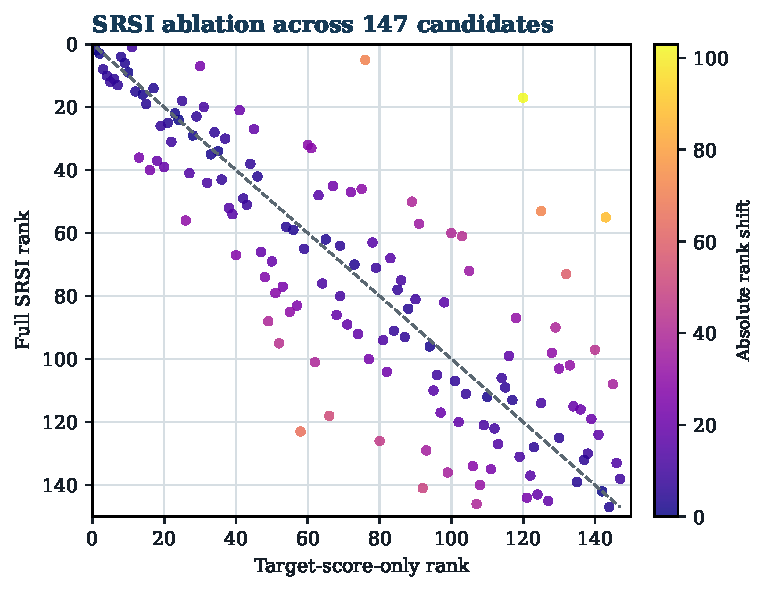
\includegraphics[width=\columnwidth]{figures/Fig_srsi_ablation.pdf}
\caption{Comparison of target-score-only and full-SRSI ranks for 147
candidates. Point color reports absolute rank shift and the diagonal
marks no change. External activity data are required to determine whether
the observed changes are beneficial.}
\label{fig:ablation}
\end{figure}

\subsection{Redocking validation of the docking protocol}
\label{sec:res-redock}

Every quantity reported above derives from AutoDock Vina scores, so the
protocol was tested against RNA--ligand complexes whose bound poses are
experimentally determined. Four were used: 8R62 and 8R63, risdiplam and
branaplam bound to the RNA duplex formed on 5$'$ splice-site
recognition; 8R8P, the splicing modifier SMN-CX bound to the RNA helix
formed on \textit{SMN2} exon 7 5$'$ splice-site recognition; and 5KX9,
a ribocil analogue bound to the FMN riboswitch, as an unrelated
RNA--ligand positive control. Each ligand was rebuilt from SMILES, so
no run began from the deposited conformer. The protocol---grid box,
exhaustiveness 32, 20 modes, five seeds---was fixed and hashed before
any RMSD was computed. Across 45 deposited receptor models and five
seeds, all 225 planned jobs completed and 4{,}488 Vina modes were
retained for symmetry-corrected analysis.

Top-ranked pose recovery was limited but informative
(Table~\ref{tab:redock}). Branaplam met the predeclared rank-1
$<2$~\AA{} criterion: its top-scored mode was 1.307~\AA{} from model 1
and 1.244~\AA{} from the closest deposited ensemble member, reproducing
17 of 21 native contacts. Risdiplam, at the same site and under the same
protocol, was not recovered at rank 1. Its top-scored mode was
12.587~\AA{} from model 1 (11.923~\AA{} ensemble minimum), shared none
of 29 model-1 native contacts, and no seed placed a sub-2~\AA{} pose
first. The unrelated riboswitch control also failed at rank 1, at
6.173~\AA{} with 27\% contact recall, so the difficulty is not peculiar
to the splice site.

The risdiplam rank-1 mismatch is diagnostically useful.
A pose within 2.478~\AA{} of the deposited ensemble \emph{was}
generated, but ranked fourteenth of twenty. Sampling approached the
neighborhood of the correct answer; scoring did not prioritize it. The
same pattern holds for SMN-CX, where the best mode of twenty reaches
1.856~\AA{} but ranks last. Even branaplam's success is fragile: only
one of five seeds ranked a sub-2~\AA{} pose first. Deposited ensemble
spread is 0.68 to 1.31~\AA{} at the median, so the deviations exceed the
experimental uncertainty by a wide margin.

\begin{table*}[!t]
\caption{Redocking Recovery Against Experimentally Determined Bound Poses}
\label{tab:redock}
\centering
\footnotesize
\setlength{\tabcolsep}{4.5pt}
\renewcommand{\arraystretch}{1.25}
\begin{tabular}{@{}llcccccc@{}}
\toprule
\textbf{PDB} & \textbf{Ligand} &
\makecell{\textbf{Rank-1 RMSD}\\\textbf{vs. model 1 (\AA)}} &
\makecell{\textbf{Rank-1 RMSD}\\\textbf{ensemble min. (\AA)}} &
\makecell{\textbf{Best sampled}\\\textbf{RMSD (\AA)}} &
\makecell{\textbf{Rank of}\\\textbf{best mode}} &
\makecell{\textbf{Contact}\\\textbf{recall}} &
\makecell{\textbf{Contact}\\\textbf{Jaccard}}\\
\midrule
8R63 & Branaplam              & 1.307  & 1.244  & 1.137 & 2  & 0.810 & 0.630\\
8R8P & SMN-CX                 & 7.169  & 6.986  & 1.856 & 20 & 0.273 & 0.162\\
5KX9 & Ribocil analogue       & 6.173  & 6.173  & 4.384 & 15 & 0.271 & 0.198\\
8R62 & Risdiplam              & 12.587 & 11.923 & 2.478 & 14 & 0.000 & 0.000\\
\bottomrule
\end{tabular}
\end{table*}

%=======================================================================
% Float barrier removed: with the single-column figures every figure now
% settles in Methods/Results on its own, and the barrier was forcing an
% early page break that left most of a page blank.

\section{Discussion}
%=======================================================================
The principal result is that SMN2-RescueDiff functioned as an end-to-end,
auditable prioritization pipeline at a scale large enough to expose both
candidate signals and method limitations. It transformed a 149{,}534-
molecule unique training set into 49{,}660 unique generated strings,
retained 40{,}477 chemically filtered molecules, completed a
five-conformer structural screen for 500 candidates, and executed
14{,}259 real Vina counter-screening jobs. The analysis then reduced the
data to a uniform $147\times97$ matrix without filling missing jobs with
synthetic scores. These are practical successes in reproducible pipeline
construction, data provenance, and large-scale RNA-screen orchestration.

The strongest candidate-level result is target-score enrichment within
the generated population. Every one of the 40 ranked candidates received
a more favorable mean \textit{SMN2} score than the median of ten
property-matched controls, with a mean gap of 0.729~kcal/mol. The result
exceeded all 2{,}000 random cohorts, and the low pairwise fingerprint
similarity and 977 scaffold labels among 1{,}000 exported molecules show
that the workflow did not reach this stage by reproducing a narrow set
of near-duplicate structures. Because a target-score-only cohort
enriched at least as strongly, the result validates the pipeline's
ability to enrich its own population for favorable target scores; it
does not establish an incremental benefit for the complete ranking rule
or prove binding.

The hard-decoy stage adds value by preventing that target-score result
from being overinterpreted. Across the top ten candidates, the weighted
mean gap spans only 0.44~kcal/mol, whereas the conservative gap spans
2.24~kcal/mol and is negative throughout. The same worst-case pattern
occurs across all 147 evaluable molecules and under the two held-out
splicing-modifier controls. Rather than treating this as a failed
pipeline, it is more accurate to treat it as a successful quality gate:
the system detected that average target--decoy separation did not survive
the strongest member of a bias-matched panel. Prior work has shown that
RNA-targeting models require careful negative examples to avoid shortcut
learning~\cite{wen2026}; the present architecture operationalizes that
principle for structural screening.

Redocking provides the necessary calibration for interpreting this
gate. Branaplam was recovered at rank 1 with 1.307~\AA{} model-1 RMSD
and 81\% contact recall, demonstrating that the fixed workflow can
recover an experimental RNA--ligand pose in at least one relevant case.
For SMN-CX and risdiplam, lower-RMSD modes were sampled but not ranked
first. Thus, the benchmark separates a sampling capability from a
scoring limitation and identifies a concrete improvement path: preserve
the sampled ensemble and add RNA-aware reranking. Until that is done,
negative conservative gaps characterize this Vina protocol, not the
biological selectivity of the molecules.

The methodological contribution is therefore the screening
architecture and its audit trail. Selectivity is evaluated in the same
workflow as target scoring rather than as a post-hoc claim; worst-case
and average separation are reported together; the target is represented
by five conformers rather than one structure; known modifiers are held
out from training; and missing jobs remain explicit. Desirability
functions use fixed prespecified windows rather than comparison-set
min--max normalization, so adding or removing a compound does not change
the meaning of an acceptance level. These choices are consistent with
RNA-targeted drug-design strategies that combine structural, chemical,
and interaction evidence rather than relying on one score
alone~\cite{haga2023},~\cite{zhou2024}.

The SRSI ablation further clarifies what the integrated ranking does.
The full ranking correlated 0.822 with target score alone and shared 33
of its top 40 molecules with the target-only ranking, while individual
rank shifts reached 103 positions. The composite therefore is neither
identical to target-only selection nor independently validated. It is a
transparent prioritization policy whose added value must ultimately be
tested against experimental labels. Likewise, attribution of a linear
standardized score primarily documents configured weights and feature
dispersion; it should not be presented as biological mechanism.

\subsection{Limitations}
\label{sec:limits}

This study is entirely computational. Vina scores, predicted rescue
scores, desirability values and SRSI values are prioritization metrics,
not measurements of exon 7 inclusion, RNA-binding affinity, cellular
activity, toxicity or therapeutic efficacy. The off-target risk index is
an index defined by this workflow, not a probability of biological
off-target activity.

The docking protocol was tested, not biologically validated.
Section~\ref{sec:res-redock} reports rank-1 recovery for one of four
benchmark complexes. This bounds every quantity in
Sections~\ref{sec:res-selectivity}, \ref{sec:res-bench}
and~\ref{sec:res-ligand}: the Vina scores, weighted and conservative
gaps, off-target risk index, desirability aggregates, and matched-control
enrichment describe this scoring function and cannot be read as RNA
binding or selectivity measurements. The direction of bias is unknown.
AutoDock Vina was parameterized on protein--ligand complexes, and the
cited assessments report limited RNA--ligand accuracy
~\cite{agarwal2023},~\cite{gunasinghe2024}. The five target conformers
are the first five deposited models of the 8R62 NMR ensemble; conformer-
level persistence of candidate contacts was not evaluated.

The splicing-rescue and contact quantities are explicit engineering
proxies, but they are not biologically calibrated. In particular,
beneficial and caution counts are fixed fractions of the global close-
contact count when corresponding landmark labels are present, rather
than nucleotide-specific contact assignments. The reported minimum U1
distance is also the global ligand--receptor minimum when a U1 label is
present. A minimum of 0.970~\AA{} may therefore reflect a steric clash,
not productive recognition. Pose support approaches its ceiling and the
occlusion term varies by only $7.5\times10^{-4}$, so these components
have limited discriminatory value despite their configured weights. The
ablation records rank effects but does not validate mechanism.

Only the ten highest-ranked candidates are tabulated in
Section~\ref{sec:res-selectivity}, but the worst-case claim is not an
extrapolation from them: the conservative gap was evaluated for every
evaluable molecule and is reported in
Section~\ref{sec:res-selectivity}. The ranking rule itself could not
have supported such an inference, because the lexicographic order is
settled in practice by the weighted gap alone, so rank position carries
no information about the conservative gap.

Raw Vina scores were compared across receptors of differing size and
composition without ligand-efficiency normalization. Because the score
scales with ligand heavy-atom count, comparisons between molecules of
different size, and selectivity gaps computed by subtracting scores
obtained on different receptors, are both susceptible to size artifacts.
The apparent target-score advantage of MolGen\_038292 over two
substantially smaller reference compounds should be regarded as
unresolved until efficiency-normalized scores are reported.

The sequence-level decoy atlas was specified at over 180{,}000 motifs,
but only 100 decoys were built as three-dimensional receptors, and 97
were available in the uniform analyzed matrix. Equal coverage across
147 molecules establishes comparability within this pilot panel; it does
not establish transcriptome-wide selectivity. The strongest-decoy
statistic is also panel-size dependent because adding receptors creates
more opportunities for an extreme score. Sensitivity across independent
panels and multiple panel sizes remains necessary.

The 400 candidate--control assignments used only 183 distinct controls,
so control reuse creates dependence not represented by a simple
candidate-level sign-flip test. The random-cohort and target-only
analyses address selection effects but do not supply an external
chemical-library control. Cluster-aware uncertainty analysis and an
external benchmark are still needed.

The generative model is unconditional and was trained on ChEMBL/ZINC
subsets; the configured R-BIND and SMMRNA sources contributed zero rows.
The run record did not capture the exact database release identifiers,
download dates, or source licenses, and novelty was approximated against
20{,}000 training fingerprints rather than the complete corpus. No
controlled n-gram, GRU, or library-sampling baseline is reported. These
limitations prevent attribution of screening performance to the
Transformer architecture or to RNA-ligand-focused training.

The most direct next step is RNA-aware reranking of the retained pose
ensembles: Table~\ref{tab:redock} shows that lower-RMSD modes for
risdiplam and SMN-CX were already sampled. A strengthened study should
also maintain a prespecified benchmark of at least 20--30 diverse
RNA--ligand complexes, report ligand-efficiency and receptor-normalized
scores, repeat the hard-decoy analysis across panel sizes, and add
experimental \textit{SMN2} splicing, direct-binding, and cellular assays
~\cite{aslesh2022},~\cite{chong2021}.

%=======================================================================
\section{Conclusion}
%=======================================================================
SMN2-RescueDiff implements a reproducible multi-stage computational
workflow combining unconditional autoregressive molecular generation,
chemical-quality and diversity filtering, five-conformer \textit{SMN2}
docking, staged human-RNA decoy counter-screening, held-out controls,
and an ablatable multi-factor ranking scheme. The audited run produced
40{,}477 filtered generated molecules, exported 1{,}000 diverse docking
candidates, completed all 2{,}500 target jobs, and assembled 14{,}259
real-Vina decoy results into a common $147\times97$ comparison matrix.
This establishes that the complete computational workflow is executable,
traceable, and capable of narrowing a large generated library without
silently imputing missing evidence.

The pipeline also produced a reproducible positive screening signal:
all 40 leading candidates had more favorable mean target scores than
their property-matched control medians, with 0.729~kcal/mol mean
enrichment and no equally large result among 2{,}000 random cohorts.
That enrichment is best interpreted as evidence that the staged workflow
can select favorable target scores within its generated population. It
is not proof of binding, and a target-only ranking performed at least as
well, so the added biological value of SRSI remains to be validated.

The hard-decoy and redocking modules strengthen the study by defining
where interpretation must stop. Favorable average target--decoy gaps did
not translate into worst-case separation, and only branaplam achieved
sub-2~\AA{} rank-1 recovery in the four-complex redocking set. At the
same time, lower-RMSD modes were sampled for SMN-CX and risdiplam,
providing a concrete route toward RNA-aware reranking rather than a need
to discard the pipeline. The resulting contribution is an auditable
candidate-prioritization architecture that produces testable molecular
hypotheses while making its calibration limits visible.

The identified molecules remain \textit{in silico} candidates. No claim
is made that they bind \textit{SMN2}, increase exon 7 inclusion, improve
cellular phenotypes, are safe, or outperform risdiplam or branaplam.
Those questions require orthogonal computational scoring and prospective
experimental validation. Within that boundary, SMN2-RescueDiff provides
a reproducible foundation for the next round of RNA-aware rescoring and
laboratory prioritization.

%=======================================================================
\section*{Acknowledgments}
The author used ChatGPT, Claude, and OpenAI Codex to assist with plotting
and analysis code, figure layout, repository auditing, and manuscript
revision in response to external critique. These tools did not generate
the underlying docking calculations. Numerical claims in this revision
were checked against the released tables, logs, and provenance records;
no missing docking value was invented or imputed. Grammarly was used for
grammar and spelling correction. The author reviewed the complete text
and takes responsibility for its claims. The author thanks Dr.~Joy Li
(Duke University) for mentorship.

\section*{Code and Data Availability}
The exact audited snapshot is commit \texttt{deacf03} on the
\texttt{real-pipeline-rigor} branch of the project repository,
\url{github.com/sakshams-cyber/SMN2-RescueDiff}. The
\texttt{reproducibility/tcbb\_2026} release contains the 100 decoy
receptors, five target receptors, prepared ligand PDBQT files, complete
score tables, per-job status records, the 741-job missingness table,
generation audit, Stage C.5 inputs, Module 5 ablation outputs, four-
complex redocking structures and tables, source manifest, and SHA-256
checksums. The release validation records Python 3.11.15, AutoDock Vina
1.2.7, Open Babel 3.2.1, and spyrmsd 0.9.0. Figure-generation code and
the manuscript source are included with this revision package.

\section*{Declarations}
\textit{Ethical approval:} Not applicable. This study is entirely
computational and involved no human participants, human data or animal
subjects.

%=======================================================================
\begin{thebibliography}{26}
\bibitem{aslesh2022}
T. Aslesh and T. Yokota, ``Restoring SMN expression: An overview of the
therapeutic developments for the treatment of spinal muscular
atrophy,'' \emph{Cells}, vol. 11, no. 3, p. 417, Jan. 2022, doi:
10.3390/cells11030417.

\bibitem{chong2021}
L. C. Chong, G. Gandhi, J. M. Lee, W. W. Y. Yeo, and S.-B. Choi, ``Drug
discovery of spinal muscular atrophy (SMA) from the computational
perspective: A comprehensive review,'' \emph{Int. J. Mol. Sci.},
vol. 22, no. 16, p. 8962, Aug. 2021, doi: 10.3390/ijms22168962.

\bibitem{strauss2022}
K. A. Strauss \emph{et al.}, ``Onasemnogene abeparvovec for
presymptomatic infants with two copies of \emph{SMN2} at risk for spinal
muscular atrophy type 1: The phase III SPR1NT trial,'' \emph{Nat. Med.},
vol. 28, no. 7, pp. 1381--1389, Jul. 2022, doi:
10.1038/s41591-022-01866-4.

\bibitem{warner2018}
K. D. Warner, C. E. Hajdin, and K. M. Weeks, ``Principles for targeting
RNA with drug-like small molecules,'' \emph{Nat. Rev. Drug Discov.},
vol. 17, no. 8, pp. 547--558, Aug. 2018, doi: 10.1038/nrd.2018.93.

\bibitem{childs2022}
J. L. Childs-Disney, X. Yang, Q. M. R. Gibaut, Y. Tong, R. T. Batey, and
M. D. Disney, ``Targeting RNA structures with small molecules,''
\emph{Nat. Rev. Drug Discov.}, vol. 21, no. 10, pp. 736--762, Oct. 2022,
doi: 10.1038/s41573-022-00521-4.

\bibitem{haga2023}
C. L. Haga and D. G. Phinney, ``Strategies for targeting RNA with small
molecule drugs,'' \emph{Expert Opin. Drug Discov.}, vol. 18, no. 2,
pp. 135--147, Feb. 2023, doi: 10.1080/17460441.2022.2111414.

\bibitem{xi2024}
W. Xi, R. Wang, L. Wang, X. Ye, M. Liu, and T. Sakurai, ``An
interpretable deep learning model predicts RNA--small molecule binding
sites,'' \emph{Future Gener. Comput. Syst.}, vol. 159, pp. 557--566,
Oct. 2024, doi: 10.1016/j.future.2024.05.029.

\bibitem{zhou2024}
Y. Zhou and S.-J. Chen, ``Advances in machine-learning approaches to
RNA-targeted drug design,'' \emph{Artif. Intell. Chem.}, vol. 2, no. 1,
p. 100053, Jun. 2024, doi: 10.1016/j.aichem.2024.100053.

\bibitem{olivecrona2017}
M. Olivecrona, T. Blaschke, O. Engkvist, and H. Chen, ``Molecular
de-novo design through deep reinforcement learning,'' \emph{J.
Cheminformatics}, vol. 9, no. 1, p. 48, Sep. 2017, doi:
10.1186/s13321-017-0235-x.

\bibitem{liu2025}
D. Liu \emph{et al.}, ``DiffMeta-RL: Reinforcement learning-guided graph
diffusion for metabolically stable molecular generation,'' \emph{J.
Chem. Inf. Model.}, vol. 65, no. 21, pp. 11746--11765, Nov. 2025, doi:
10.1021/acs.jcim.5c02060.

\bibitem{popova2018}
M. Popova, O. Isayev, and A. Tropsha, ``Deep reinforcement learning for
de novo drug design,'' \emph{Sci. Adv.}, vol. 4, no. 7, p. eaap7885,
Jul. 2018, doi: 10.1126/sciadv.aap7885.

\bibitem{wen2026}
Y. Wen, Y. Han, and D. Wang, ``Overcoming shortcut learning in
RNA-small molecule modeling via bias-matched decoys and structure-aware
network design,'' \emph{J. Chem. Inf. Model.}, vol. 66, no. 11,
pp. 6403--6417, Jun. 2026, doi: 10.1021/acs.jcim.6c00360.

\bibitem{karroucha2025}
W. Karroucha, C. Oliver, V. Stoven, and V. Mallet, ``Machine learning
for RNA-targeting drug design,'' Dec. 17, 2025, arXiv:2512.15645, doi:
10.48550/arXiv.2512.15645.

\bibitem{agarwal2023}
R. Agarwal, Rajitha Rajeshwar T., and J. C. Smith, ``Comparative
assessment of pose
prediction accuracy in RNA--ligand docking,'' \emph{J. Chem. Inf.
Model.}, vol. 63, no. 23, pp. 7444--7452, Dec. 2023, doi:
10.1021/acs.jcim.3c01533.

\bibitem{gunasinghe2024}
K. K. J. Gunasinghe, I. R. H. Ginjom, H. S. San, T. Rahman, and X. C.
Wezen, ``Can current molecular docking methods accurately predict RNA
inhibitors?,'' \emph{J. Chem. Inf. Model.}, vol. 64, no. 15,
pp. 5954--5963, Aug. 2024, doi: 10.1021/acs.jcim.4c00235.

\bibitem{allen2026}
T. E. H. Allen, M. Bonnet, and R. T. Khan, ``Generative chemistry
platform for small molecules targeting RNA: A case study for chemical
optimization,'' May 12, 2026, \emph{Bioinformatics}, doi:
10.64898/2026.05.08.723908.

\bibitem{zdrazil2024}
B. Zdrazil \emph{et al.}, ``The ChEMBL database in 2023: A drug
discovery platform spanning multiple bioactivity data types and time
periods,'' \emph{Nucleic Acids Res.}, vol. 52, no. D1,
pp. D1180--D1192, Jan. 2024, doi: 10.1093/nar/gkad1004.

\bibitem{irwin2020}
J. J. Irwin \emph{et al.}, ``ZINC20---A free ultralarge-scale chemical
database for ligand discovery,'' \emph{J. Chem. Inf. Model.}, vol. 60,
no. 12, pp. 6065--6073, Dec. 2020, doi: 10.1021/acs.jcim.0c00675.

\bibitem{baell2010}
J. B. Baell and G. A. Holloway, ``New substructure filters for removal
of pan assay interference compounds (PAINS) from screening libraries and
for their exclusion in bioassays,'' \emph{J. Med. Chem.}, vol. 53,
no. 7, pp. 2719--2740, Apr. 2010, doi: 10.1021/jm901137j.

\bibitem{bickerton2012}
G. R. Bickerton, G. V. Paolini, J. Besnard, S. Muresan, and A. L.
Hopkins, ``Quantifying the chemical beauty of drugs,'' \emph{Nat.
Chem.}, vol. 4, no. 2, pp. 90--98, Feb. 2012, doi: 10.1038/nchem.1243.

\bibitem{krenn2020}
M. Krenn, F. H\"ase, A. Nigam, P. Friederich, and A. Aspuru-Guzik,
``Self-referencing embedded strings (SELFIES): A 100\% robust molecular
string representation,'' \emph{Mach. Learn. Sci. Technol.}, vol. 1,
no. 4, p. 045024, Dec. 2020, doi: 10.1088/2632-2153/aba947.

\bibitem{trott2010}
O. Trott and A. J. Olson, ``AutoDock Vina: Improving the speed and
accuracy of docking with a new scoring function, efficient optimization,
and multithreading,'' \emph{J. Comput. Chem.}, vol. 31, no. 2,
pp. 455--461, Jan. 2010, doi: 10.1002/jcc.21334.

\bibitem{eberhardt2021}
J. Eberhardt, D. Santos-Martins, A. F. Tillack, and S. Forli, ``AutoDock
Vina 1.2.0: New docking methods, expanded force field, and Python
bindings,'' \emph{J. Chem. Inf. Model.}, vol. 61, no. 8,
pp. 3891--3898, Aug. 2021, doi: 10.1021/acs.jcim.1c00203.

\bibitem{li2026}
J. Li, S. Zhou, C. Liu, Q. Wang, T. Liu, and M. Zang,
``Fourier-enhanced Kolmogorov--Arnold network with attention for
drug--target interaction prediction,'' \emph{IEEE Trans. Comput. Biol.
Bioinforma.}, vol. 23, no. 3, pp. 1393--1404, May 2026, doi:
10.1109/TCBBIO.2026.3681464.

\bibitem{rezaei2022}
M. A. Rezaei, Y. Li, D. Wu, X. Li, and C. Li, ``Deep learning in drug
design: Protein-ligand binding affinity prediction,'' \emph{IEEE/ACM
Trans. Comput. Biol. Bioinform.}, vol. 19, no. 1, pp. 407--417,
Jan. 2022, doi: 10.1109/TCBB.2020.3046945.

\bibitem{yuan2014}
J. Yuan, W. Wu, C. Xie, G. Zhao, Y. Zhao, and R. Chen, ``NPInter v2.0:
An updated database of ncRNA interactions,'' \emph{Nucleic Acids Res.},
vol. 42, no. D1, pp. D104--D108, Jan. 2014, doi: 10.1093/nar/gkt1057.
\end{thebibliography}

\begin{IEEEbiographynophoto}{Saksham Srivastava}
is a student at Saint Francis High School, Mountain View, CA, USA. He
works on computational biology and machine learning for RNA-targeted
drug design, and developed the SMN2-RescueDiff pipeline described here.
\end{IEEEbiographynophoto}

\end{document}
